\documentclass{beamer}
\usetheme{CambridgeUS}
\usecolortheme{dolphin}
\usepackage{hyperref}
\usepackage{multimedia}

% set colors
\definecolor{myNewColorA}{RGB}{126,12,110}
\definecolor{myNewColorB}{RGB}{165,85,154}
\definecolor{myNewColorC}{RGB}{203,158,197}
\setbeamercolor*{palette primary}{bg=myNewColorC}
\setbeamercolor*{palette secondary}{bg=myNewColorB, fg = white}
\setbeamercolor*{palette tertiary}{bg=myNewColorA, fg = white}
\setbeamercolor*{titlelike}{fg=myNewColorA}
\setbeamercolor*{title}{bg=myNewColorA, fg = white}
\setbeamercolor*{item}{fg=myNewColorA}
\setbeamercolor*{caption name}{fg=myNewColorA}

\title{Helion}
\subtitle{Fúzió más megközelítése}
\author[Péter Bence]{Péter Bence Gábor\\X89O8X}
\institute{Széchenyi István Egyetem}
\date{2023. Május 9.}

\begin{document}
\titlepage


\begin{frame}
    \frametitle{Tartalom}
    \tableofcontents
\end{frame}


\section{Bevezetés}
\begin{frame}
    \frametitle{Bevezetés}
    \begin{figure}
        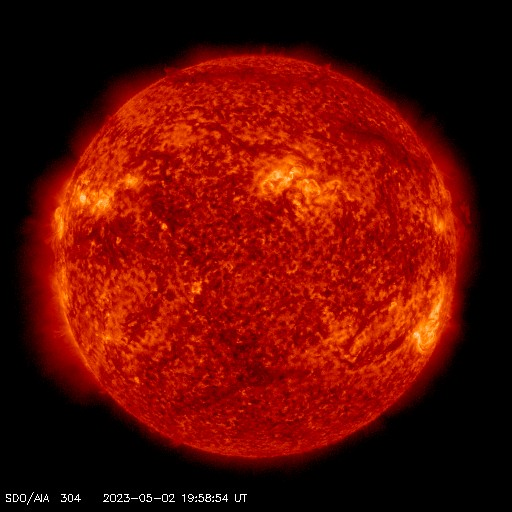
\includegraphics[scale=0.30]{latest_512_0304.jpg}
        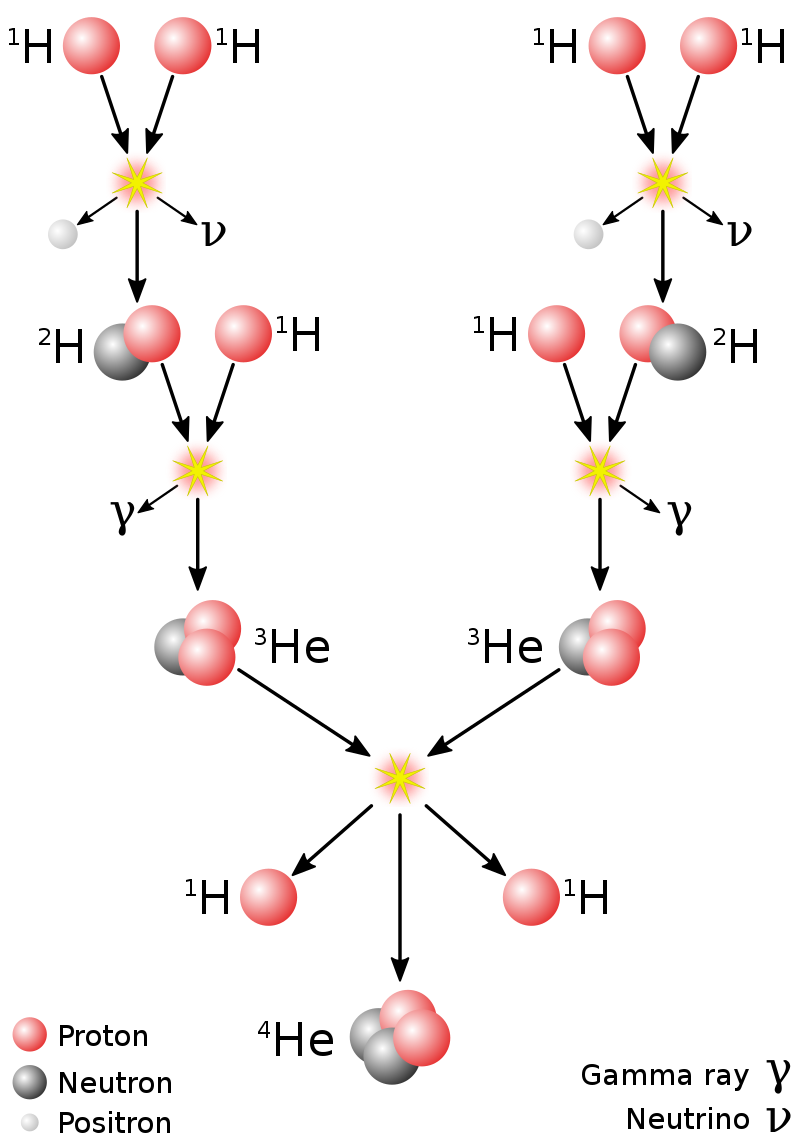
\includegraphics[scale=0.13]{800px-Fusion_in_the_Sun.svg.png}
    \end{figure} 
\end{frame}


\subsection{Fúzió}
\begin{frame}
    \frametitle{Fúzió}
    \begin{figure}
        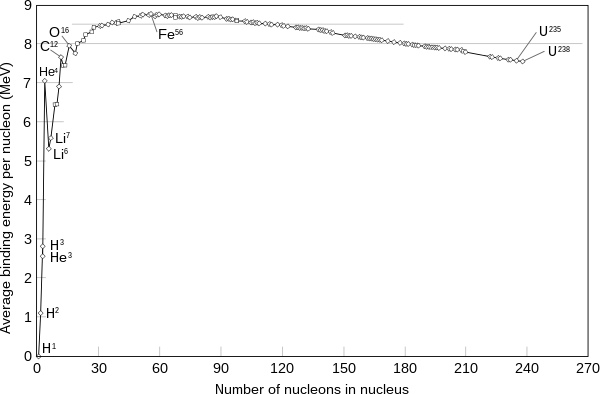
\includegraphics[scale=0.5]{Binding_energy_curve_-_common_isotopes.svg.png}
    \end{figure} 
\end{frame}


\subsection{Tokamak}
\begin{frame}
    \frametitle{Tokamak}
    \begin{figure}
        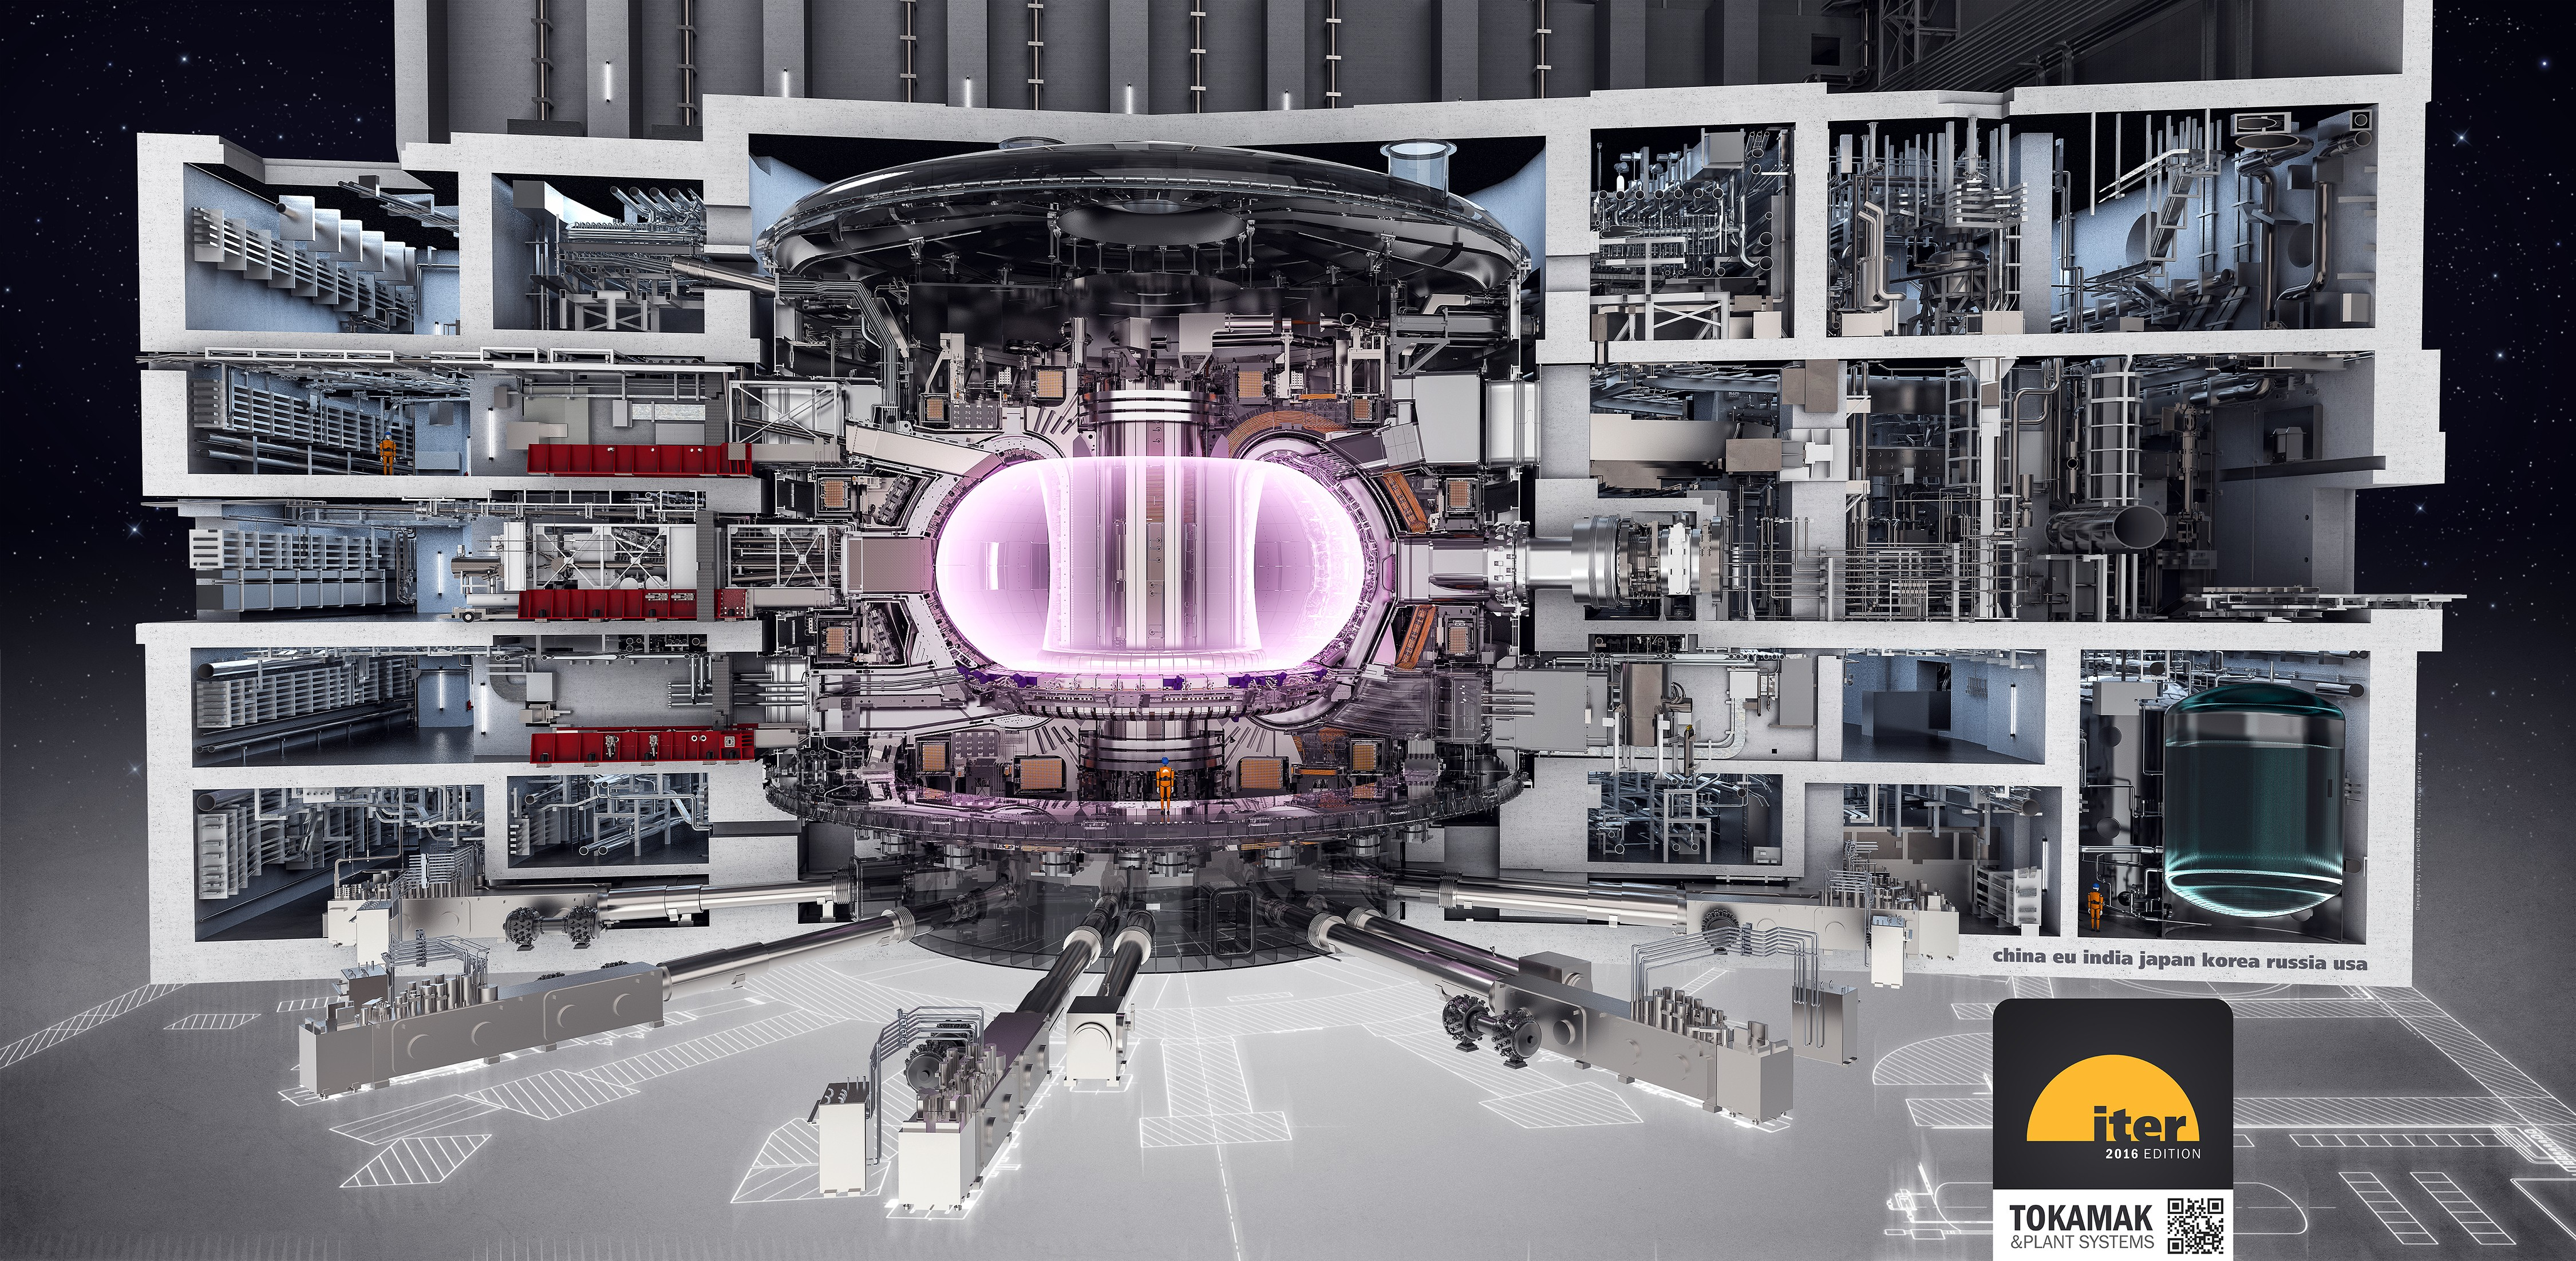
\includegraphics[scale=0.043]{iter.jpeg}
        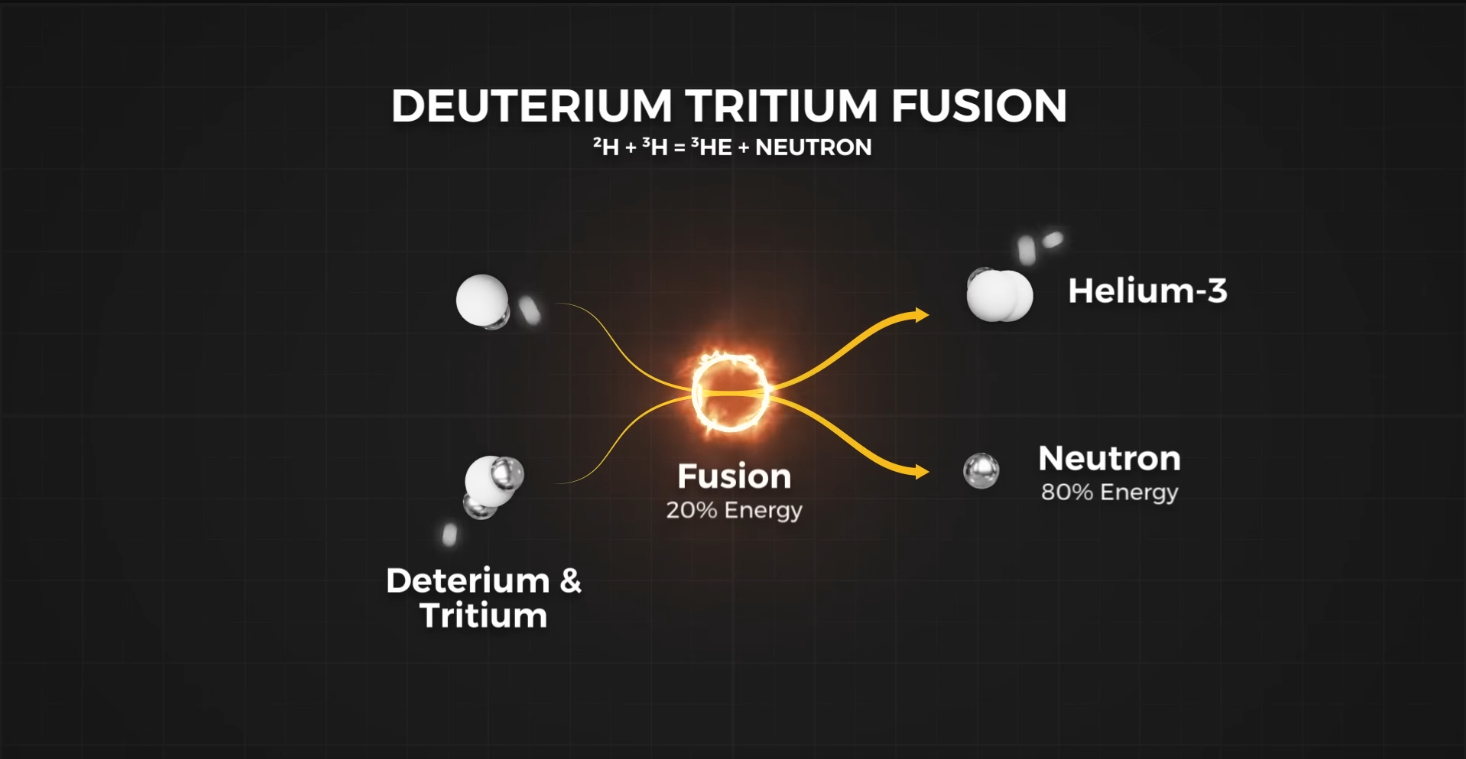
\includegraphics[scale=0.135]{deut_trit_v2.png}
    \end{figure} 
\end{frame}


\section{Helion}
\begin{frame}
    \frametitle{Helion}
    \begin{columns}
        \column{0.3\textwidth}
        \begin{itemize}
            \item Magán cég az USA-ban
            \item Alapítvás éve: 2013
            \item CEO: Dr. David Kirtley
            \item Legújabb prototípus: Trenta
        \end{itemize}
        \column{0.7\textwidth}
        \begin{figure}
            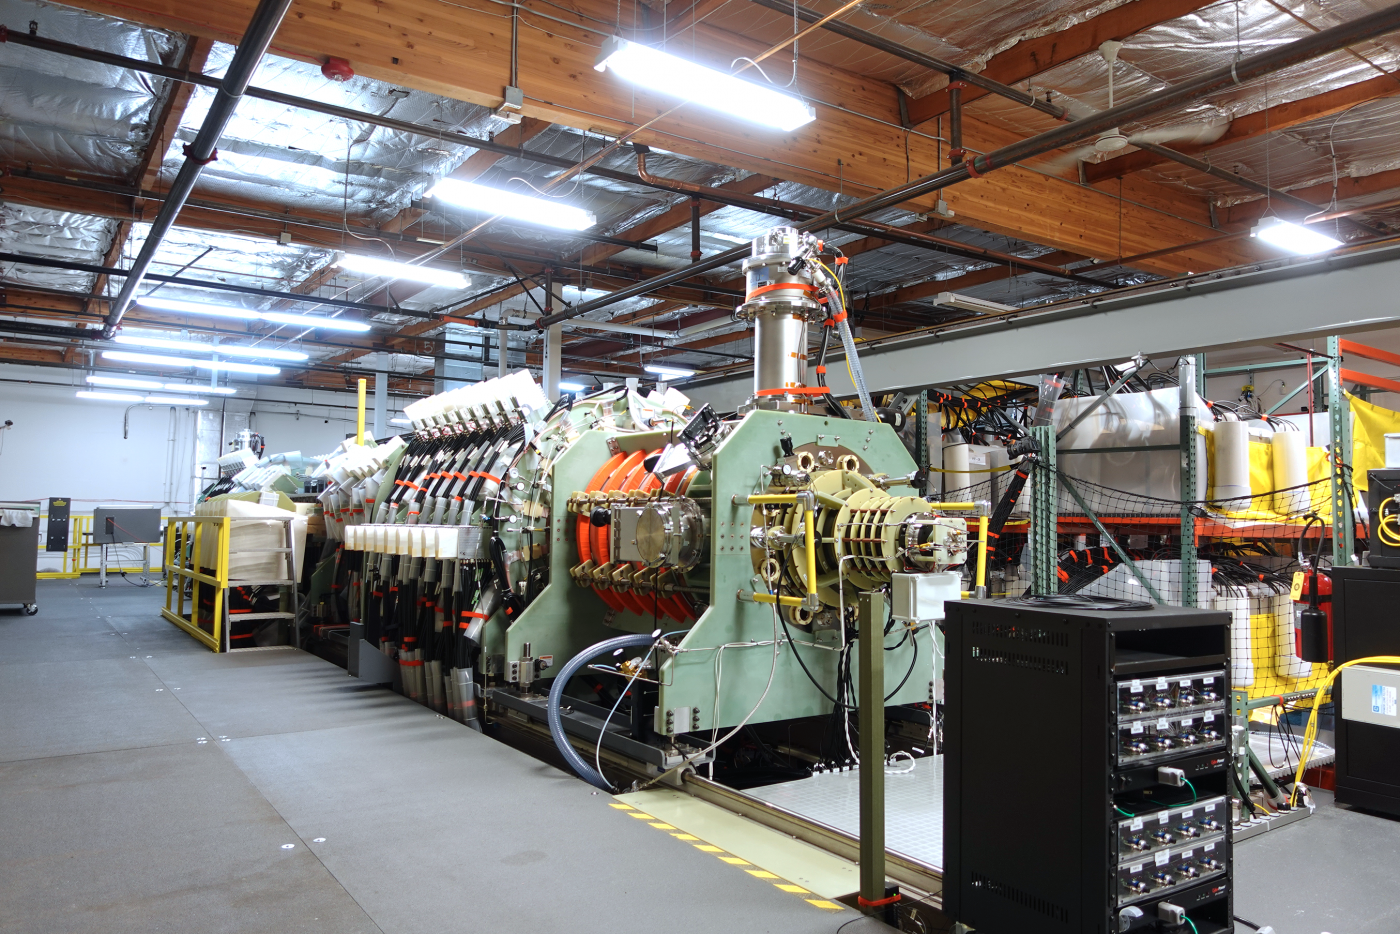
\includegraphics[scale=0.2]{trenta-1-1400x934.png}
        \end{figure}    
    \end{columns}
\end{frame}

\subsection{Működési elv}
\begin{frame}
    \frametitle{Működési elv}
    \begin{columns}
        \column{0.3\textwidth}
        \begin{itemize}
            \footnotesize
            \item Elektromágnes
            \item Field-Reverse Configuration
            \item Tekercsenként $10^5A$
            \item Elért hőmérséklet: $10^8K$
        \end{itemize}
        \column{0.7\textwidth}
        \movie[showcontrols=true, loop=true]{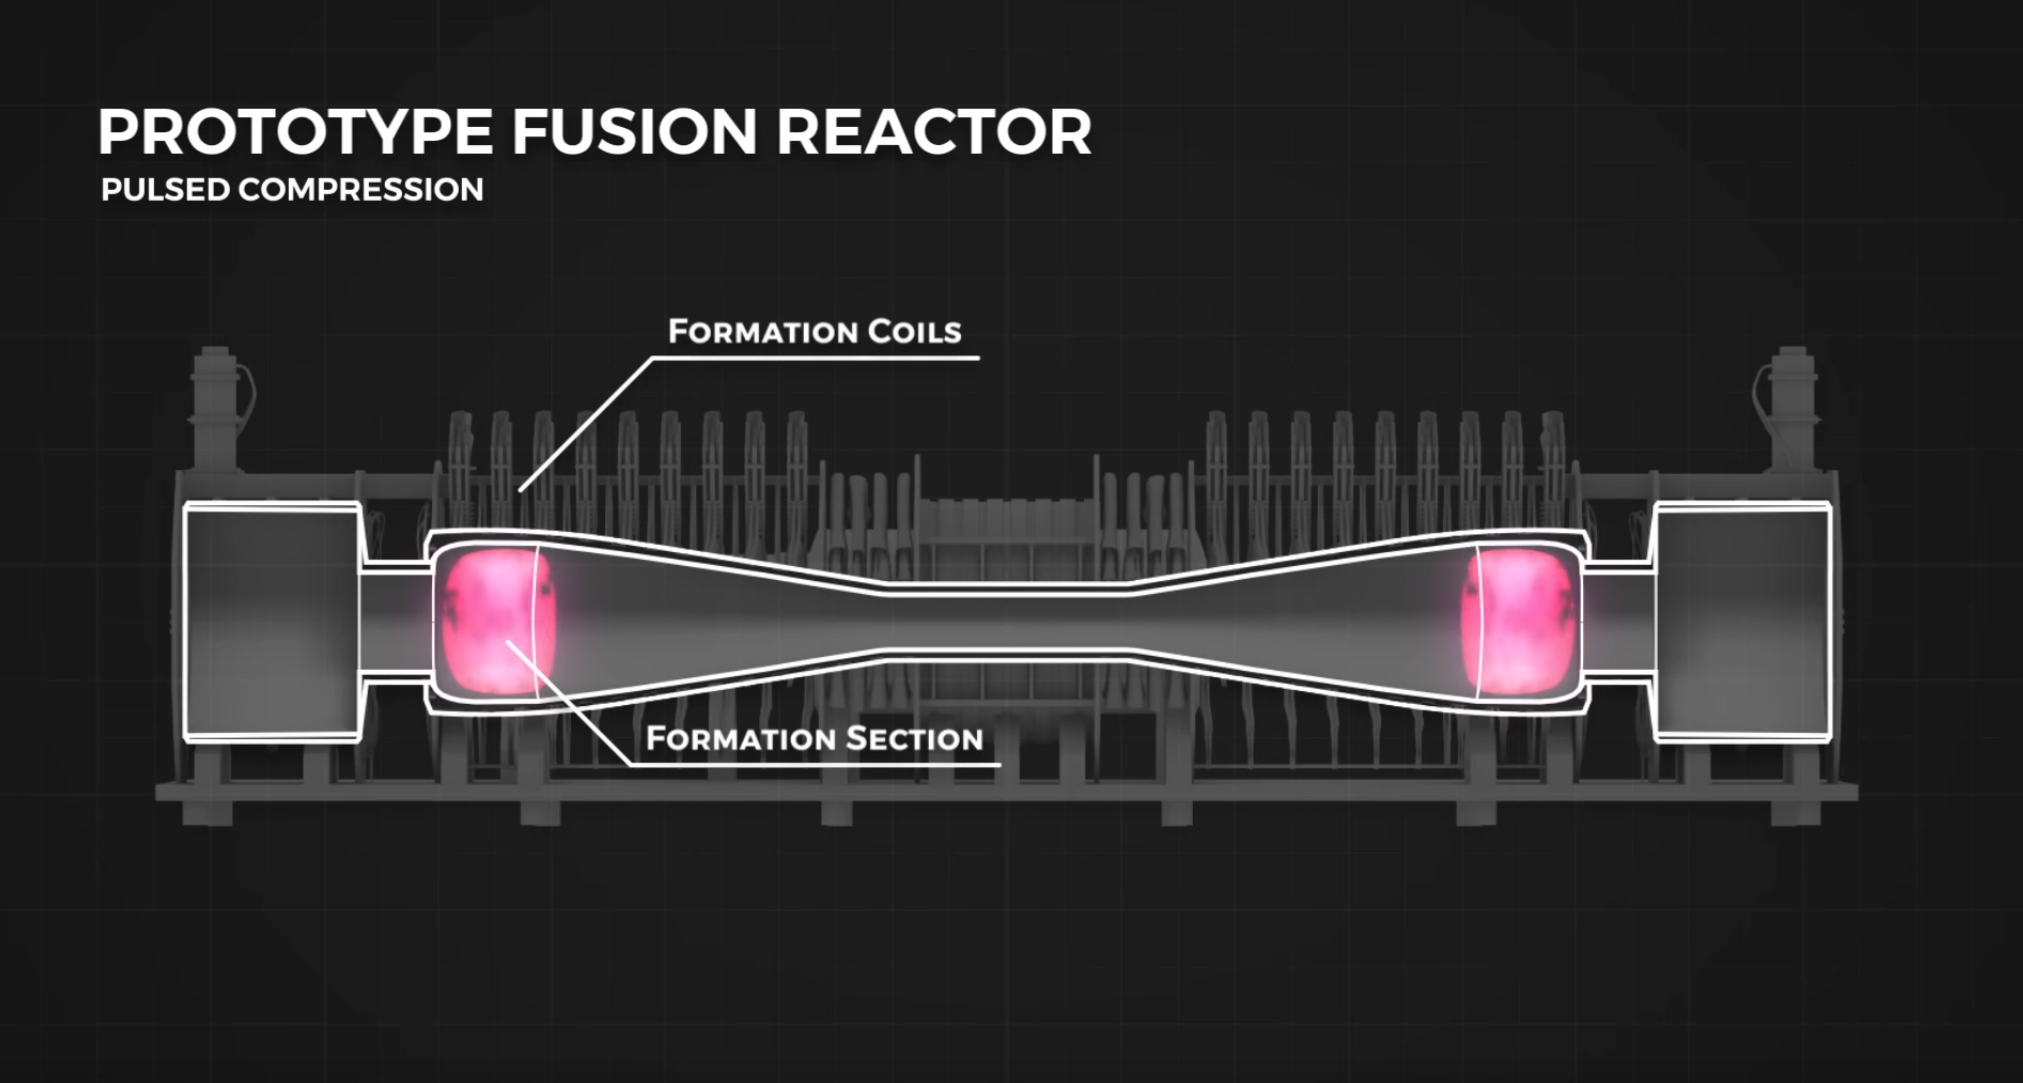
\includegraphics[scale=0.11]{helion_fusion_thumbnail.png}}{helion_fusion_video.mp4}   
    \end{columns}
\end{frame}
\begin{frame}
    \frametitle{Field-Reverse Configuration}
    \begin{itemize}
        \item Tórusz alak elérése elektromágnesekkel
        \item Plazma egybetartása
    \end{itemize}
    \begin{figure}
        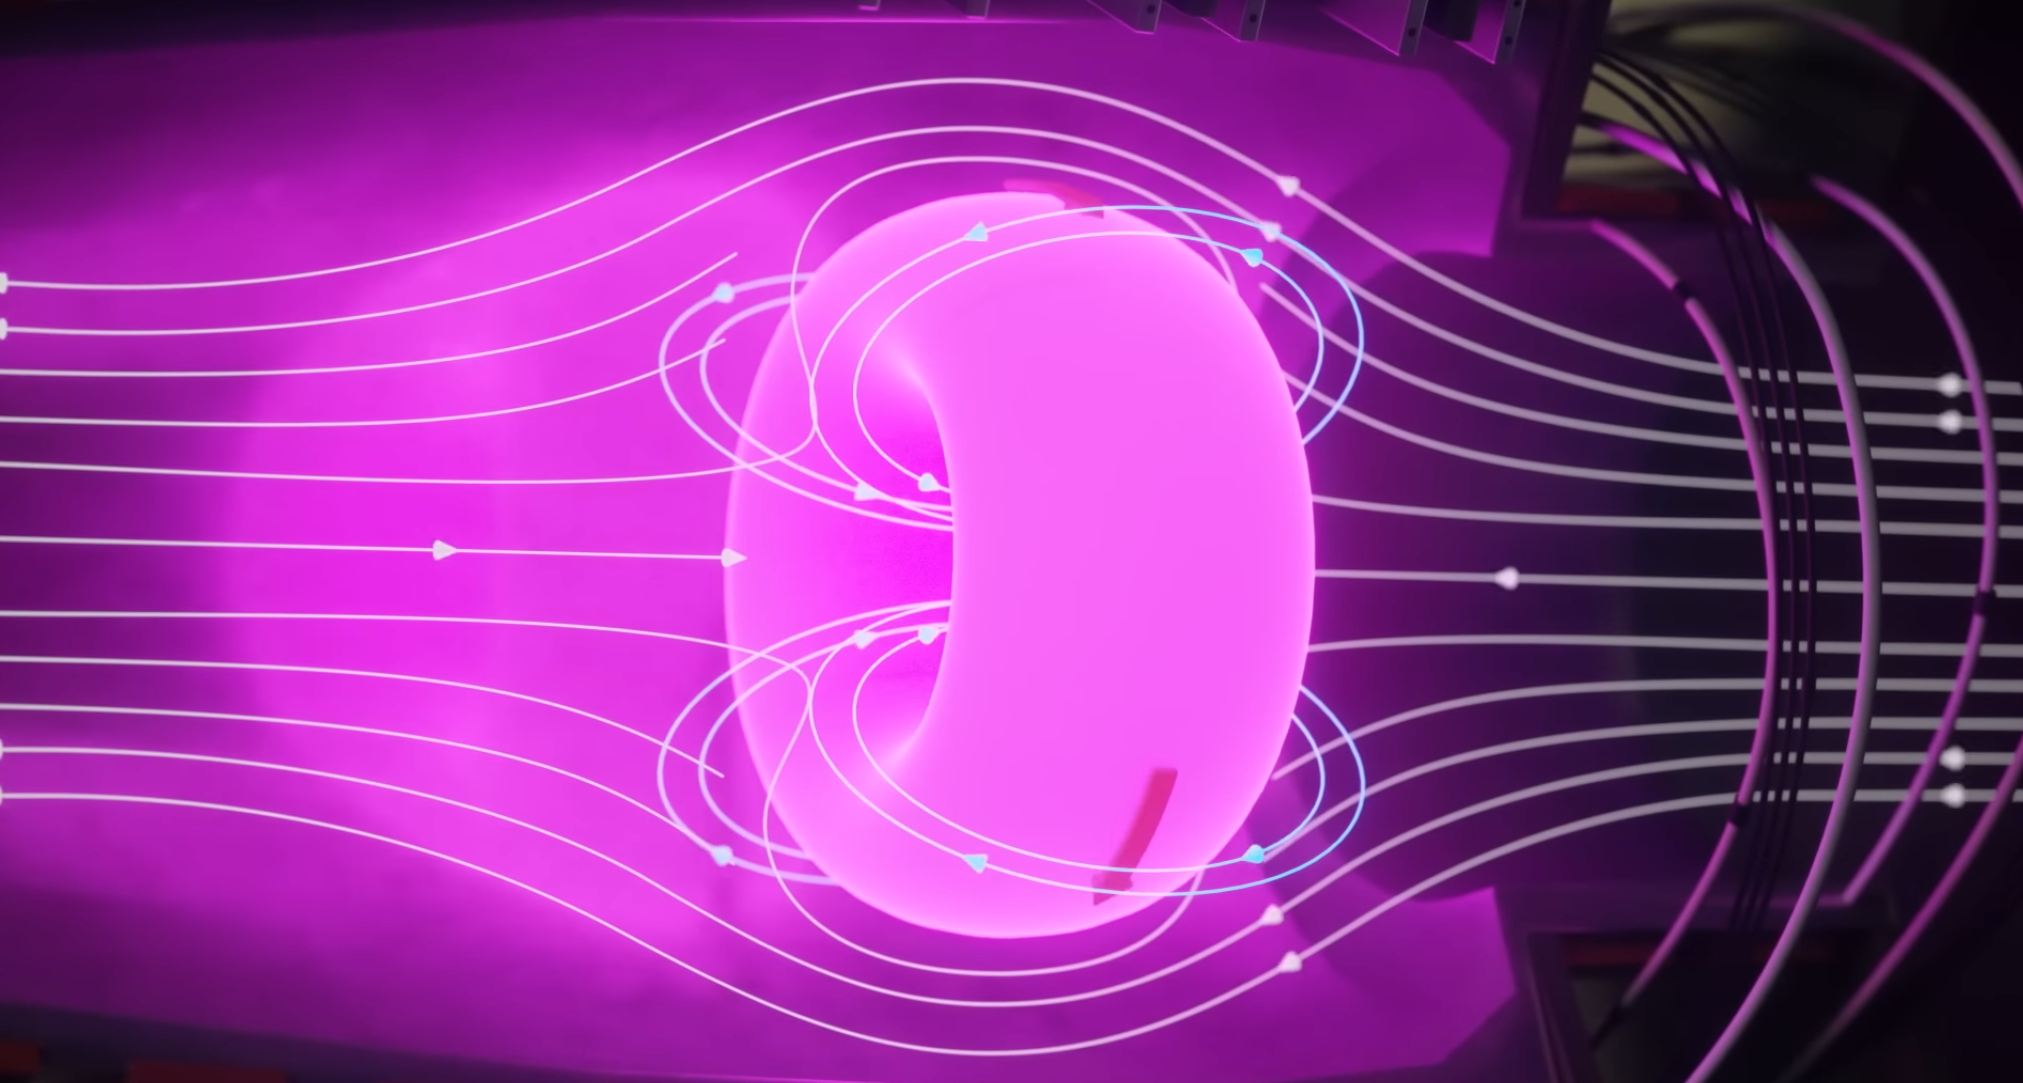
\includegraphics[scale=0.15]{field_reverse_config.png}
    \end{figure}
\end{frame}


\subsection{Fúzió}
\begin{frame}
    \frametitle{Deuterium + Deuterium}
    \begin{columns}
        \column{0.5\textwidth}
        \begin{figure}
            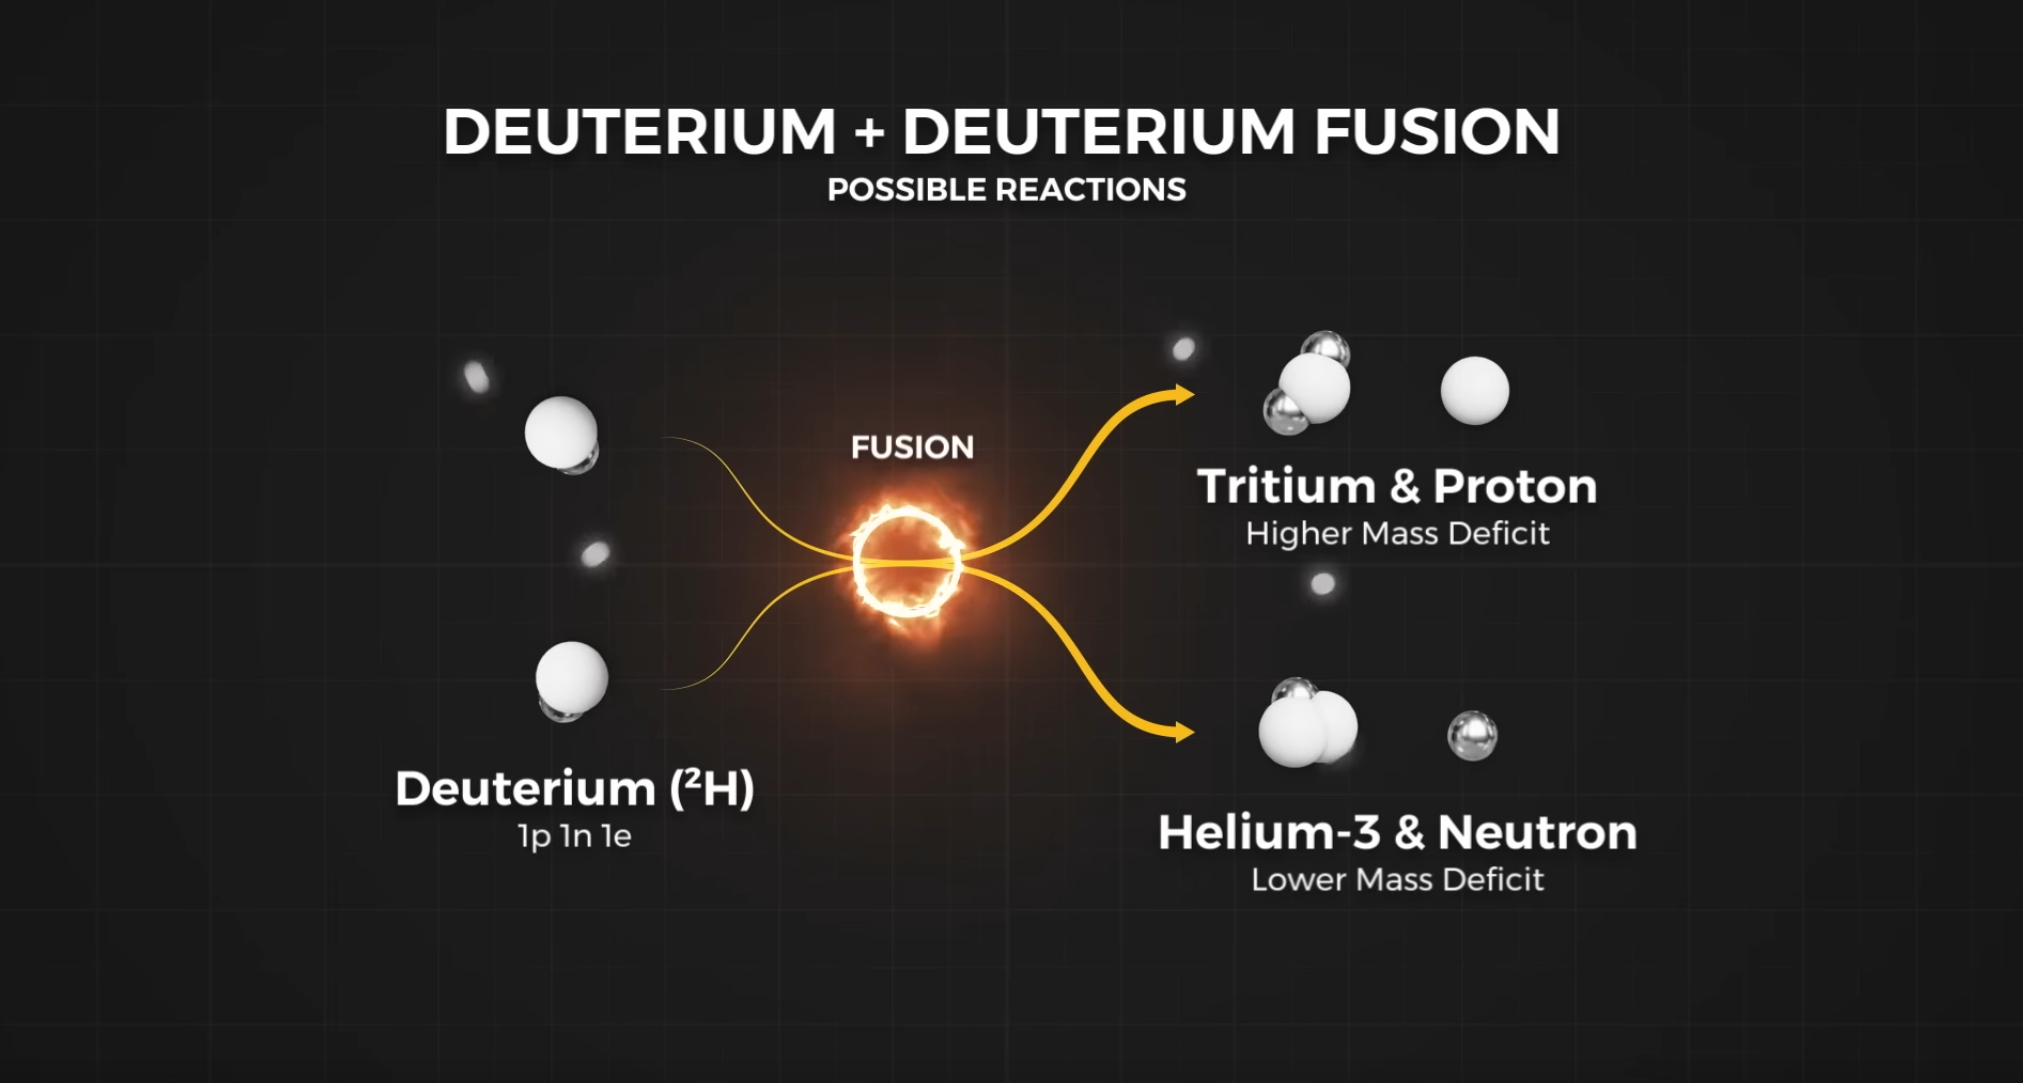
\includegraphics[scale=0.12]{d_d_fusion.png}
        \end{figure}   
        \column{0.5\textwidth}
        \begin{figure}
            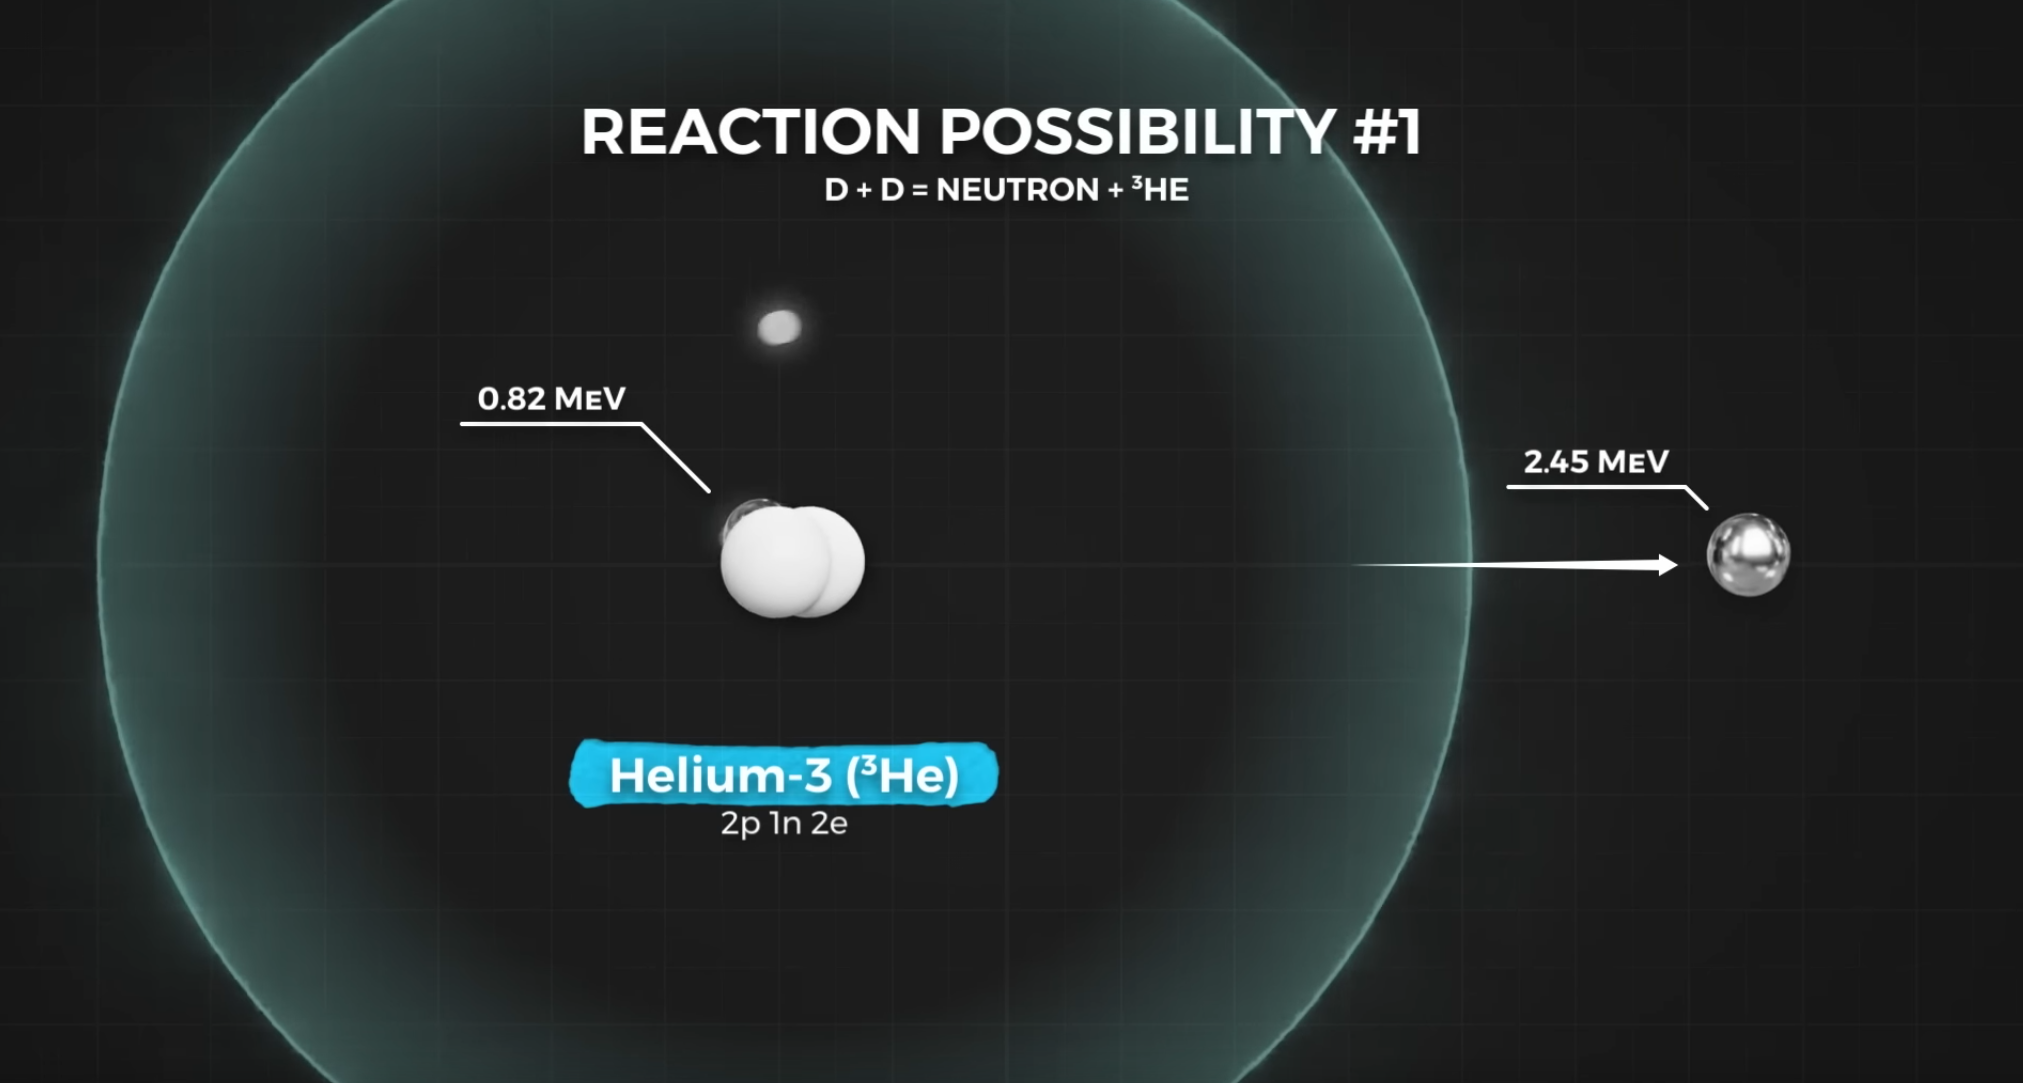
\includegraphics[scale=0.07]{d_d_fusion_possibility_1.png}
            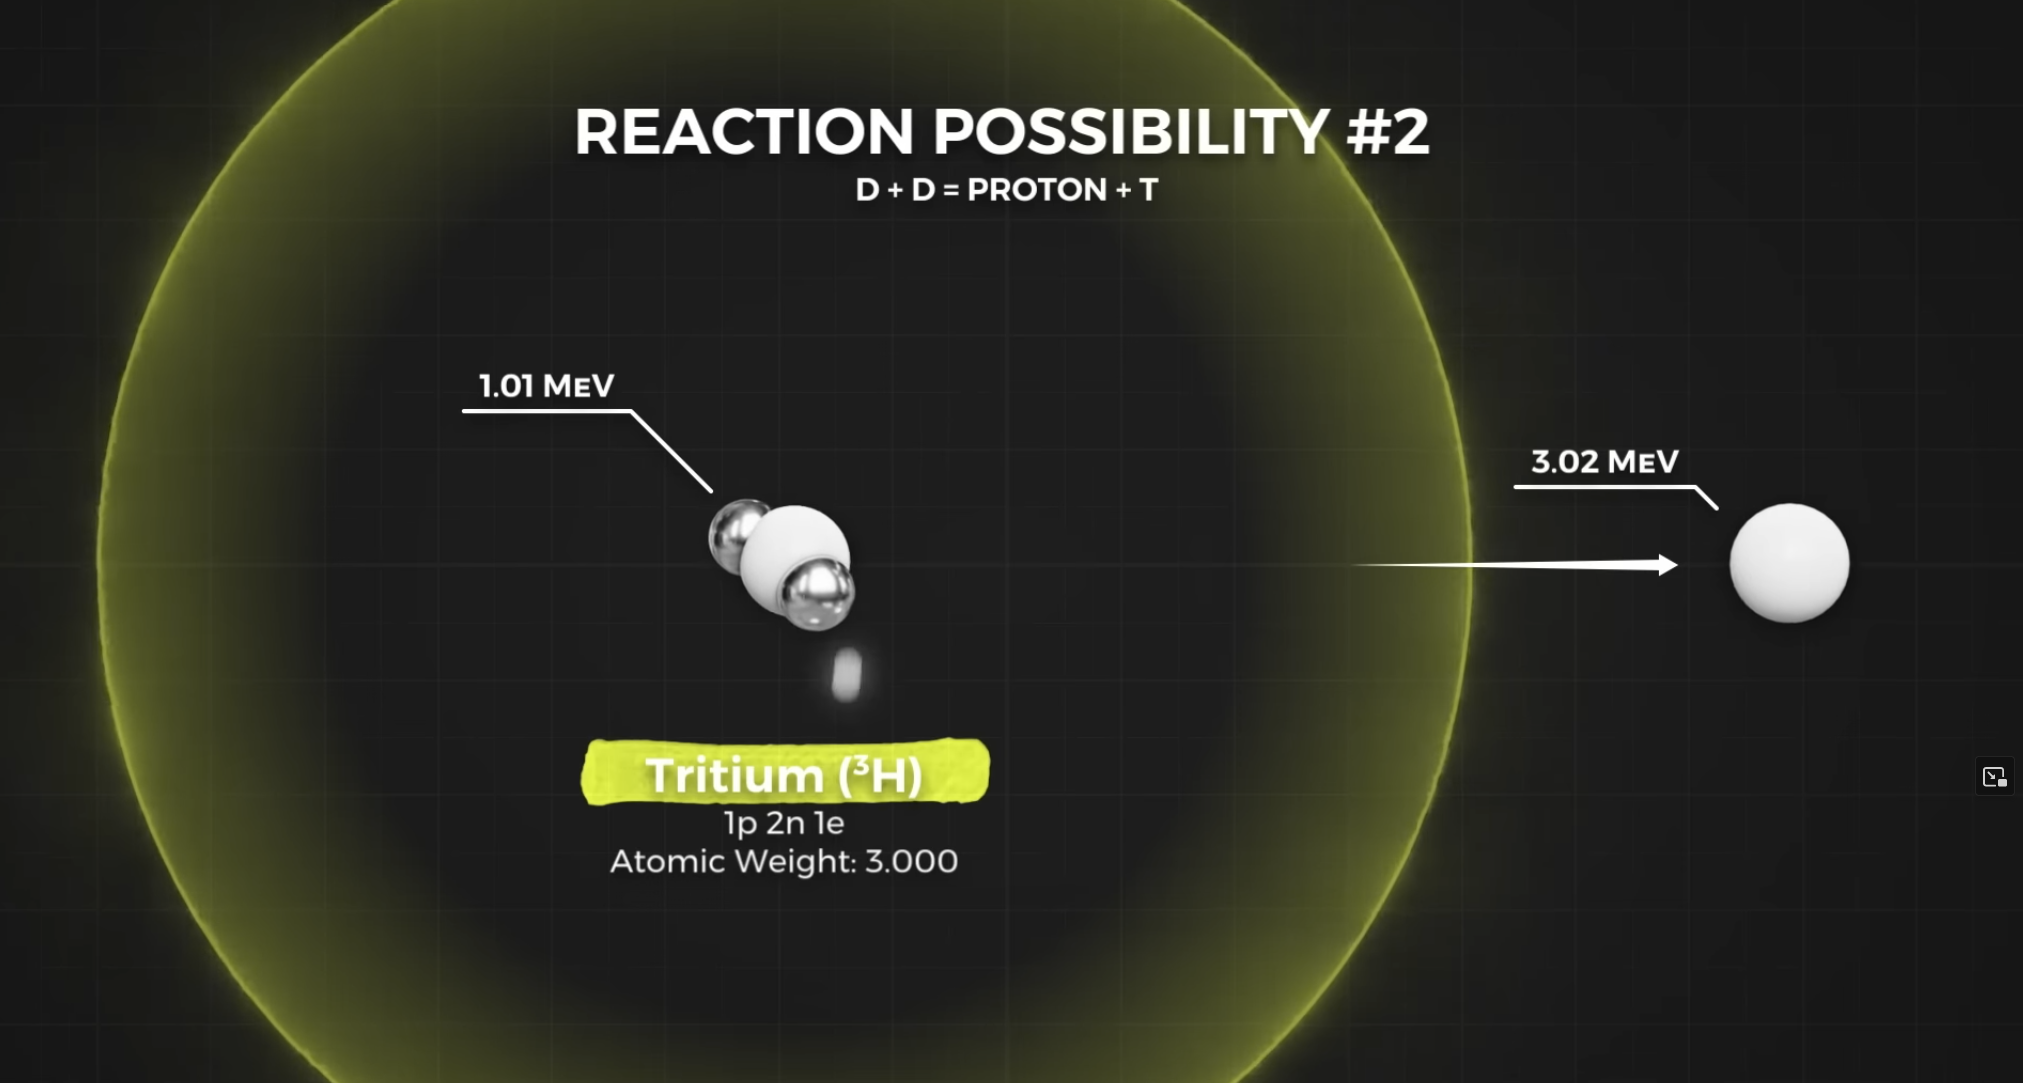
\includegraphics[scale=0.07]{d_d_fusion_possibility_2.png}
        \end{figure}   
    \end{columns}
\end{frame}
\begin{frame}
    \frametitle{Deuterium + Helium-3}
    \begin{figure}
        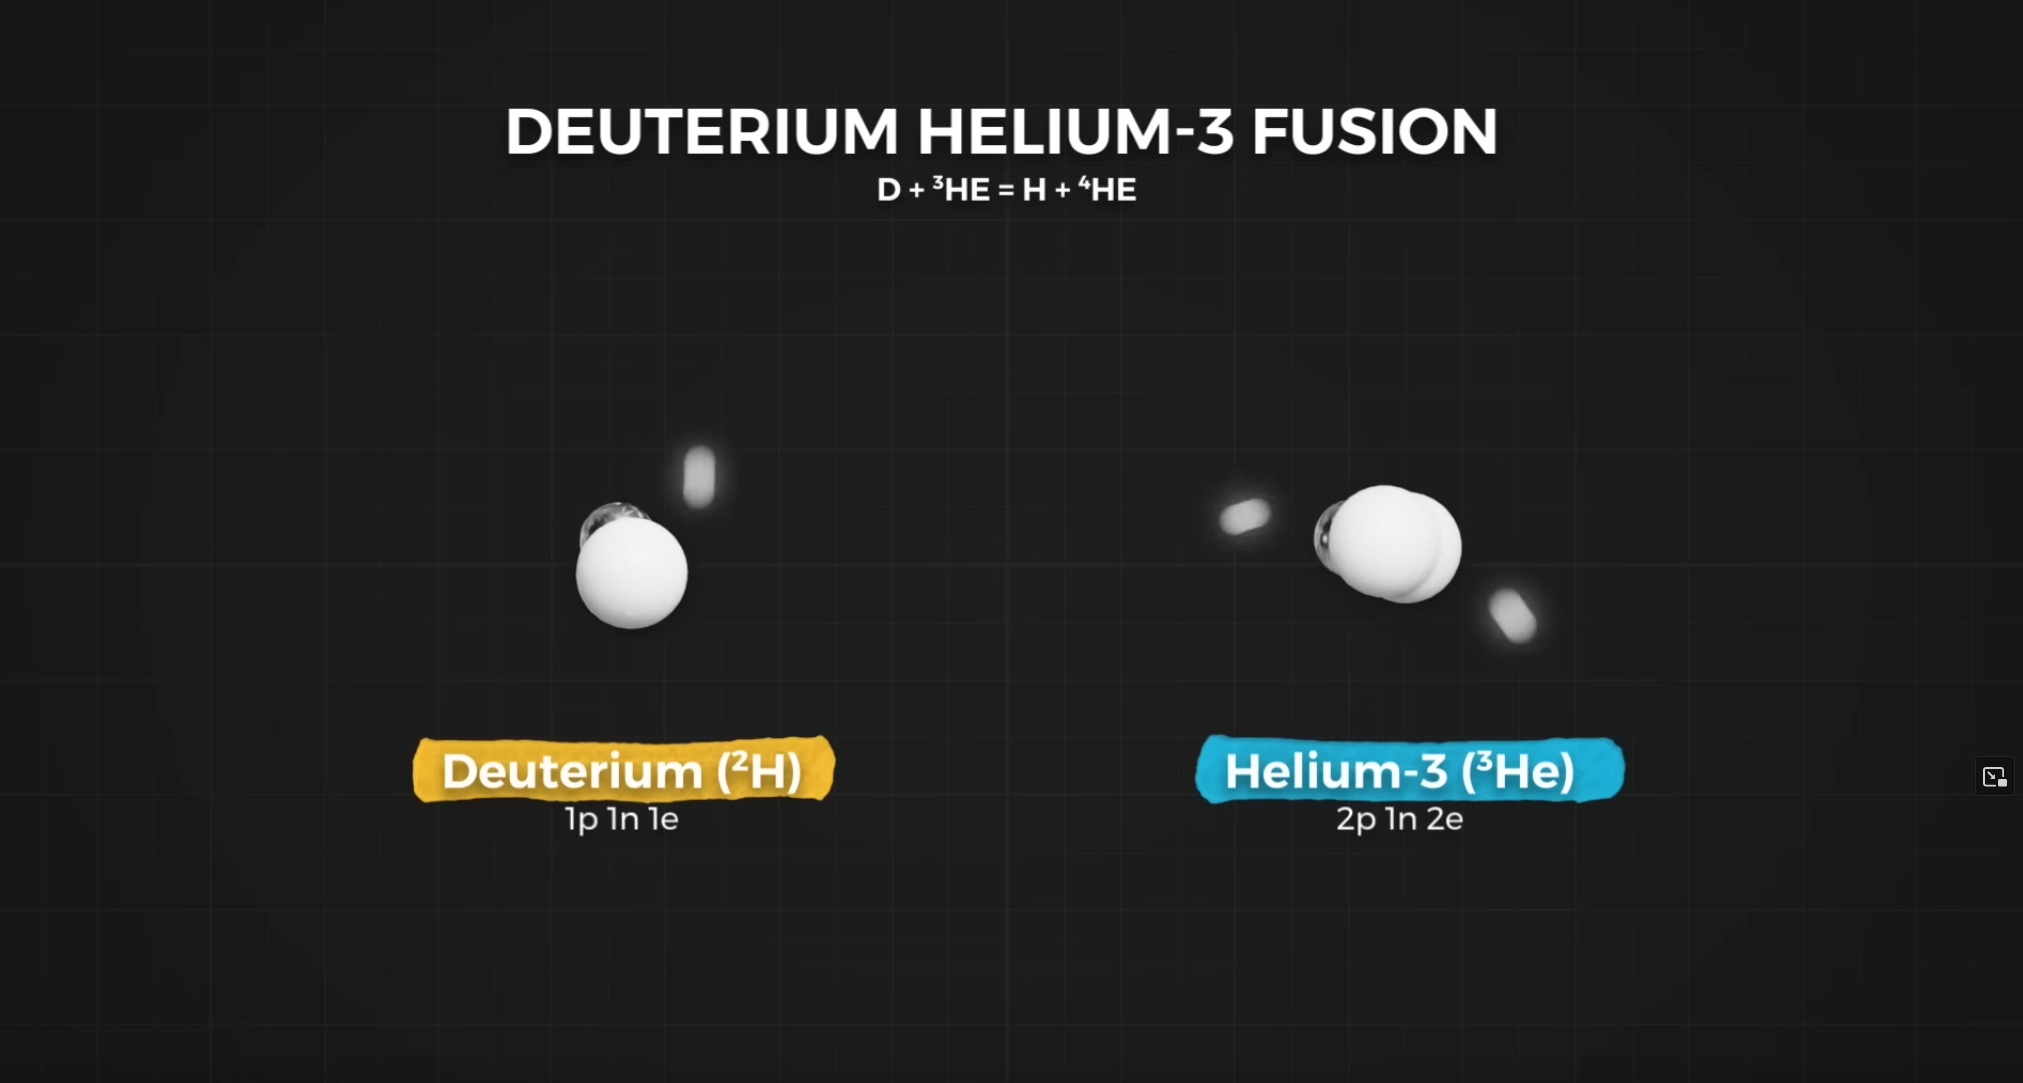
\includegraphics[scale=0.09]{d_h3_fusion.png}
        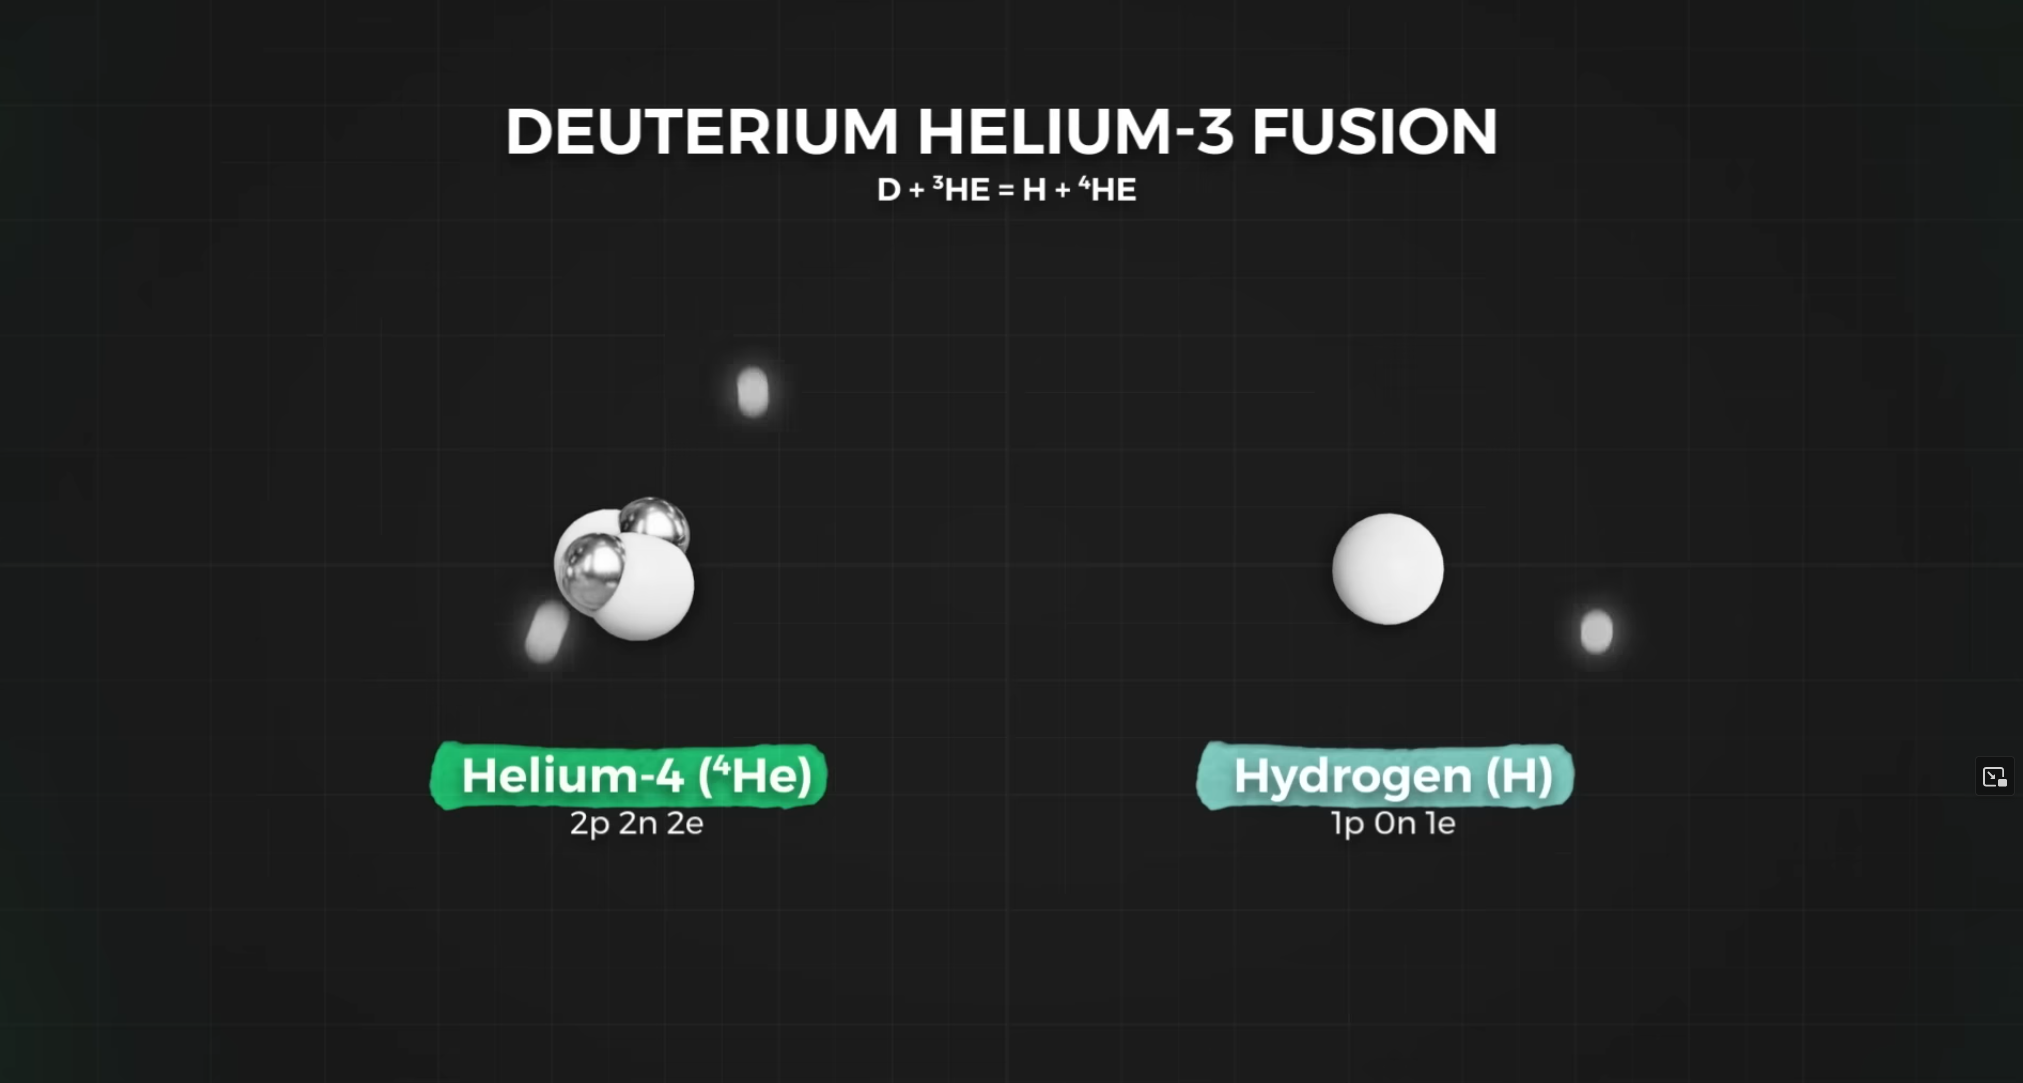
\includegraphics[scale=0.09]{d_h3_fusion_2.png}
    \end{figure}
\end{frame}

\subsection{Áram termelés}
\begin{frame}
    \frametitle{Áram termelés}
    

\end{frame}

\end{document}